\section{Testvorbereitung}
Wir w�hlen die InnoDB als Speichermaschine aus, da sie die Transaktionssicherheit gew�hrleistet und sich dadurch f�r das Betreiben eines Webshops am besten eignet. 
Jede Versuchsreihe besteht aus vier Testl�ufen zu je einem Use Case. Am Anfang  werden Testdaten mit einer  bestimmten Anzahl von Kunden, einer konstanten Anzahl von Produkten (1000) ,konstanten Anzahl von Warenk�rben pro Kunde(5) und genauso einer konstanten Anzahl von Produkten pro Warenkorb(5) generiert. Die Anzahl der Kunden erh�ht sich mit jedem Testlauf. In jeder Versuchsreihe werden die vier verschiedenen Use Cases betrachtet, die durch eine unterschiedliche SELECT-Anweisung an die MySQL-Datenbank realisiert werden:
\subsection{SELECT-Anweisungen}
\begin{enumerate}
\item \textbf{Use Case 1: Welches Produkt wurde wie oft gekauft?}
\begin{verbatim}
SELECT adbc.Produkt.Name, COUNT(*)
FROM adbc.Produkt, adbc.Warenkorb_has_Produkt
WHERE adbc.Produkt.PRODUKT_ID = 
      adbc.Warenkorb_has_Produkt.Produkt_PRODUKT_ID
GROUP BY adbc.Produkt.Name;
\end{verbatim}
\item \textbf{Wieviel Umsatz wurde von wem in bestimmtem Zeitraum generiert?}
\begin{verbatim}
SELECT adbc.kunde.Name, SUM(adbc.produkt.Preis)
FROM adbc.kunde,adbc.Produkt, 
     adbc.Warenkorb, 
     adbc.Warenkorb_has_Produkt
WHERE produkt.PRODUKT_ID = warenkorb_has_produkt.Produkt_PRODUKT_ID 
    AND warenkorb_has_produkt.Warenkorb_WARENKORB_ID 
        = warenkorb.WARENKORB_ID
    AND warenkorb.Kunde_KUNDE_ID = kunde.KUNDE_ID    
    AND (warenkorb_has_produkt.Datum BETWEEN
         '2011-01-01' AND '2011-03-01')
GROUP BY adbc.kunde.Name;
\end{verbatim}
\item \textbf{Wie viele Kunden haben in bestimmten Zeitraum bestellt?}
\begin{verbatim}
SELECT COUNT(DISTINCT(adbc.kunde.KUNDE_ID))
FROM adbc.Kunde, adbc.Warenkorb, adbc.warenkorb_has_produkt
WHERE warenkorb.Kunde_KUNDE_ID = kunde.KUNDE_ID
AND warenkorb.WARENKORB_ID = 
    warenkorb_has_produkt.Warenkorb_WARENKORB_ID
AND warenkorb_has_produkt.Datum = '2011-01-01';
\end{verbatim}
\item \textbf{Wie viel Umsatz wurde an den ersten drei Tagen der ersten drei Monate generiert?}
\begin{verbatim}
SELECT adbc.kunde.Name, SUM(adbc.produkt.Preis)
FROM adbc.kunde,adbc.Produkt, 
     adbc.Warenkorb, 
     adbc.Warenkorb_has_Produkt
WHERE produkt.PRODUKT_ID = 
      warenkorb_has_produkt.Produkt_PRODUKT_ID 
AND warenkorb_has_produkt.Warenkorb_WARENKORB_ID = 
		warenkorb.WARENKORB_ID
AND warenkorb.Kunde_KUNDE_ID = kunde.KUNDE_ID
AND ((warenkorb_has_produkt.Datum = '2011-01-01')
OR   (warenkorb_has_produkt.Datum = '2011-01-05')
OR   (warenkorb_has_produkt.Datum = '2011-01-09')    
OR   (warenkorb_has_produkt.Datum = '2011-02-02')
OR   (warenkorb_has_produkt.Datum = '2011-02-06')    
OR   (warenkorb_has_produkt.Datum = '2011-02-10')
OR   (warenkorb_has_produkt.Datum = '2011-03-10')
OR   (warenkorb_has_produkt.Datum = '2011-03-14')    
OR   (warenkorb_has_produkt.Datum = '2011-03-18'))      
GROUP BY adbc.kunde.Name;
\end{verbatim}
\end{enumerate}
\subsection{EXPLAIN-Anweisung}
Bei den SQL-Abfragen stellten wir bei jeder SELECT-Anweisung ein EXPLAIN davor, um n�tzliche Informationen zum Ausf�hrungsplan des Optimierers zu erhalten. Die EXPLAIN-Anweisung liefert u.a. Daten dar�ber, ob die Indizes auch wirklich benutzt wurden, in welcher Reihenfolge die Tabellen verkn�pft werden sowie weitere Informationen, die helfen sollen die SELECT-Anweisungen zu beschleunigen.  
\subsection{EXPLAIN PARTITIONS-Anweisung}
Diese Anweisung liefert zus�tzlich Informationen �ber die verwendeten Partitionen. Man kann sie jedoch nur auf RANGE- oder LIST-partitionierte Tabellen verwenden. Bei KEY- oder HASH-Partitionen ist sie unbrauchbar, da automatisch alle Partitionen ausgegeben werden. 

\section{Testdurchf�hrung}

blabla
\subsection{Kalt- und Warmstart ohne Index}
\begin{figure}[htp]
\centering
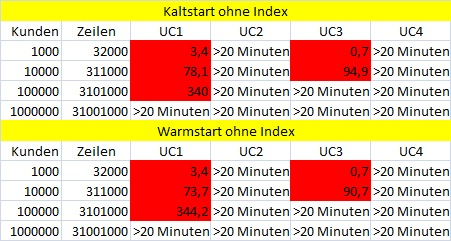
\includegraphics[width=1\textwidth]{Christof/Bilder/KaltWarm.jpg}
\caption{Kalt- und Warmstart}
\label{fig:KaltWarm}
\end{figure}



